\newpage
\section{Podsumowanie}
Zdecydowaliśmy się na porównanie wyników dla największych badanych macierzy (o wymiarach 528x528 dla pierwszej grupy i 640x640 dla drugiej grupy) i bloków o wymiarach 8x8 i 16x16. W przypadku wersji 4. wybraliśmy tę z pobraniem do rejestru, ze względu na lepsze czasy wykonania.

\begin{table}[H]
\centering
\begin{tabular}{|c|c|c|c|c|c|}
\hline
Rozwiązanie & Rozmiar bloku & Czas & GFLOPS & GIPS & CGMA \\ \hline
\multirow{2}{*}{Wersja 1} & 8x8 & 1345.355 & 0.219 & 0.03774 & 5.333 \\ \cline{2-6}
& 16x16 & 349.936 & 0.841 & 0.14509 & 8.000 \\ \hline
\multirow{2}{*}{Wersja 2} & 8x8 & 38.574 & 7.632 & 0.08095 & 21.178 \\ \cline{2-6}
& 16x16 & 36.721 & 8.017 & 0.08248 & 32.267 \\ \hline
\multirow{2}{*}{Wersja 3} & 8x8 & 7.666 & 38.402 & 0.18043 & 127.765 \\ \cline{2-6}
& 16x16 & 4.075 & 72.246 & 0.30390 & 510.593 \\ \hline
\end{tabular}
\caption{Porównanie pierwszej grupy rozwiązań -- macierz 528x528.}
\end{table}

\begin{figure}[H]

\begin{minipage}[c]{0.46\textwidth}
\centering

\resizebox{\textwidth}{!}{%
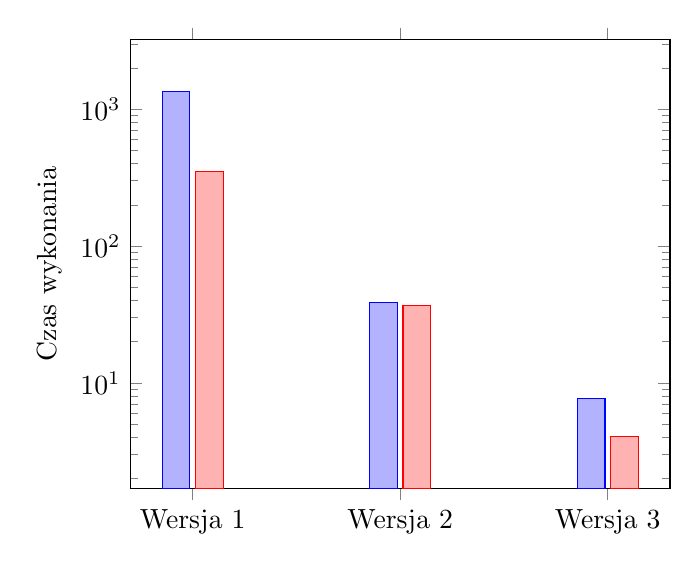
\begin{tikzpicture}
\begin{axis}[
  ybar,%=5pt,
  ylabel=Czas wykonania,
  ymode=log,
  log origin=infty,
  enlargelimits=0.15,
  xtick=data,
  symbolic x coords={Wersja 1, Wersja 2, Wersja 3}
]
\addplot 
  coordinates {%
    (Wersja 1, 1345.355)
    (Wersja 2, 38.574)
    (Wersja 3, 7.666)
  };

\addplot 
  coordinates {%
    (Wersja 1, 349.936)
    (Wersja 2, 36.721) 
    (Wersja 3, 4.075)
  };

\end{axis}
\end{tikzpicture}
}

\vspace{18pt}

\resizebox{\textwidth}{!}{%
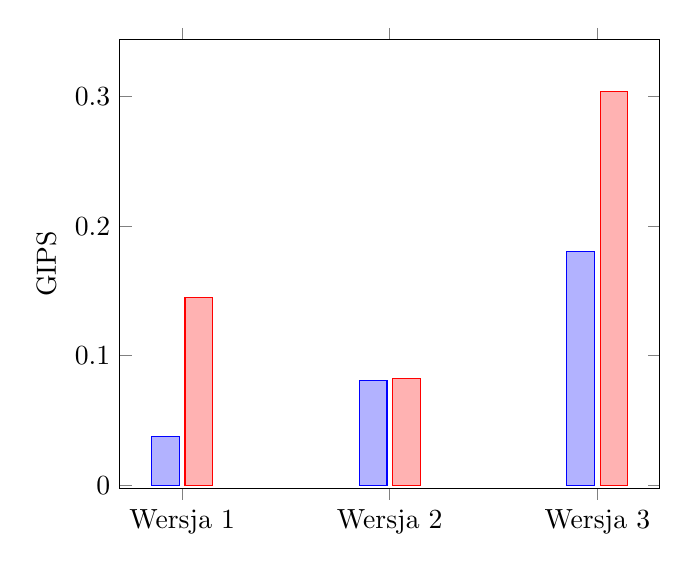
\begin{tikzpicture}
\begin{axis}[
  ybar,%=5pt,
  ylabel=GIPS,
  %ymode=log,
  log origin=infty,
  enlargelimits=0.15,
  xtick=data,
  symbolic x coords={Wersja 1, Wersja 2, Wersja 3}
]
\addplot 
  coordinates {%
    (Wersja 1, 0.03774)
    (Wersja 2, 0.08095)
    (Wersja 3, 0.18043)
  };

\addplot 
  coordinates {%
    (Wersja 1, 0.14509)
    (Wersja 2, 0.08248) 
    (Wersja 3, 0.30390)
  };

\end{axis}
\end{tikzpicture}
}
\end{minipage}
\qquad
\begin{minipage}[c]{0.46\textwidth}
\centering

\resizebox{\textwidth}{!}{%
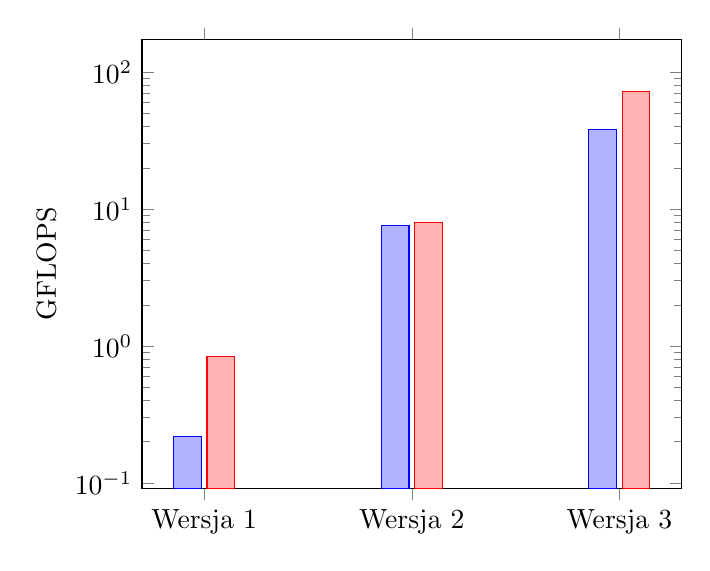
\begin{tikzpicture}
\begin{axis}[
  ybar,%=5pt,
  ylabel=GFLOPS,
  ymode=log,
  log origin=infty,
  enlargelimits=0.15,
  xtick=data,
  symbolic x coords={Wersja 1, Wersja 2, Wersja 3}
]
\addplot 
  coordinates {%
    (Wersja 1, 0.219)
    (Wersja 2, 7.632)
    (Wersja 3, 38.402)
  };

\addplot 
  coordinates {%
    (Wersja 1, 0.841)
    (Wersja 2, 8.017) 
    (Wersja 3, 72.246)
  };

\end{axis}
\end{tikzpicture}
}

\vspace{18pt}

\resizebox{\textwidth}{!}{%
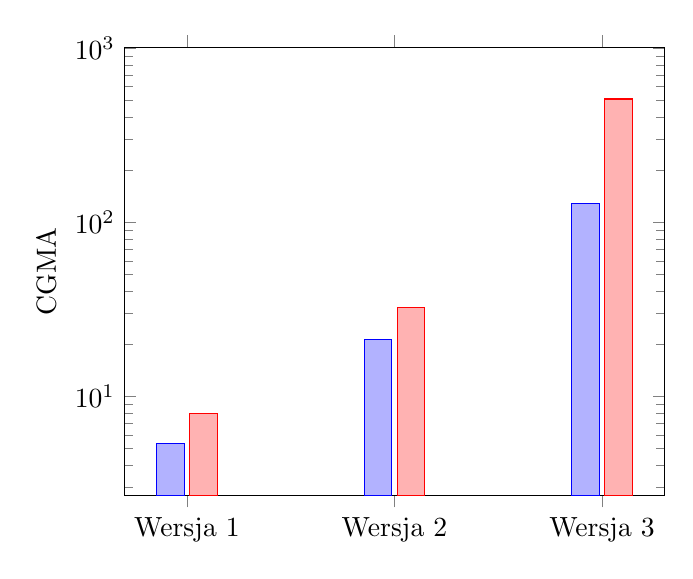
\begin{tikzpicture}
\begin{axis}[
  ybar,%=5pt,
  ylabel=CGMA,
  ymode=log,
  log origin=infty,
  enlargelimits=0.15,
  xtick=data,
  symbolic x coords={Wersja 1, Wersja 2, Wersja 3}
]
\addplot 
  coordinates {%
    (Wersja 1, 5.333)
    (Wersja 2, 21.178)
    (Wersja 3, 127.765)
  };

\addplot 
  coordinates {%
    (Wersja 1, 8.000)
    (Wersja 2, 32.267) 
    (Wersja 3, 510.593)
  };

\end{axis}
\end{tikzpicture}
}
\end{minipage}

\caption{Porównanie pierwszej grupy rozwiązań -- macierz 528x528.}

\end{figure}

\begin{table}[H]
\centering
\begin{tabular}{|c|c|c|c|c|c|}
\hline
Rozwiązanie & Rozmiar bloku & Czas & GFLOPS & GIPS & CGMA \\ \hline
\multirow{2}{*}{Wersja 3} & 8x8 & 13.820 & 37.938 & 0.1775 & 127.760 \\ \cline{2-6}
& 16x16 & 7.301 & 71.812 & 0.2989 & 510.723 \\ \hline
\multirow{2}{*}{Wersja 4} & 8x8 & 13.950 & 37.583 & 0.1815 & 126.499 \\ \cline{2-6}
& 16x16 & 7.356 & 71.269 & 0.3013 & 500.764 \\ \hline
\multirow{2}{*}{Wersja 5} & 8x8 & 12.047 & 43.520 & 0.1538 & 255.393 \\ \cline{2-6}
& 16x16 & 10.632 & 49.314 & 0.1909 & 1310.720 \\ \hline
\end{tabular}
\caption{Porównanie drugiej grupy rozwiązań -- macierz 640x640.}
\end{table}

\begin{figure}[H]

\begin{minipage}[c]{0.46\textwidth}
\centering

\resizebox{\textwidth}{!}{%
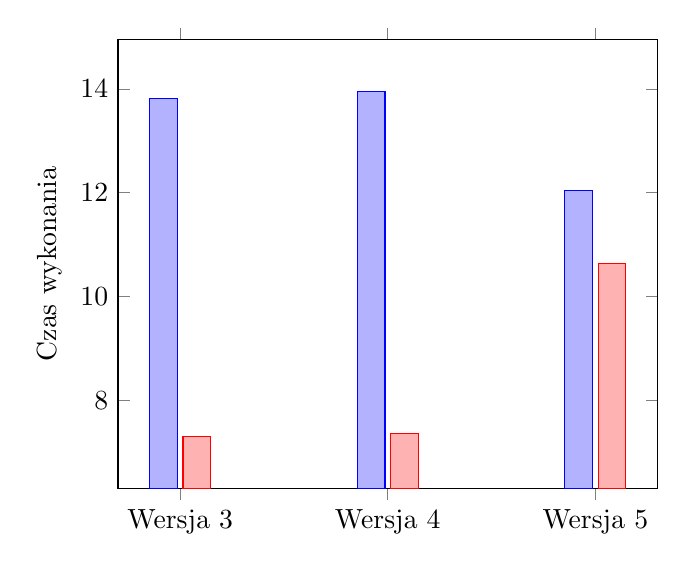
\begin{tikzpicture}
\begin{axis}[
  ybar,%=5pt,
  ylabel=Czas wykonania,
  %ymode=log,
  log origin=infty,
  enlargelimits=0.15,
  xtick=data,
  symbolic x coords={Wersja 3, Wersja 4, Wersja 5}
]
\addplot 
  coordinates {%
    (Wersja 3, 13.820)
    (Wersja 4, 13.950)
    (Wersja 5, 12.047)
  };

\addplot 
  coordinates {%
    (Wersja 3, 7.301)
    (Wersja 4, 7.356) 
    (Wersja 5, 10.632)
  };

\end{axis}
\end{tikzpicture}
}

\vspace{18pt}

\resizebox{\textwidth}{!}{%
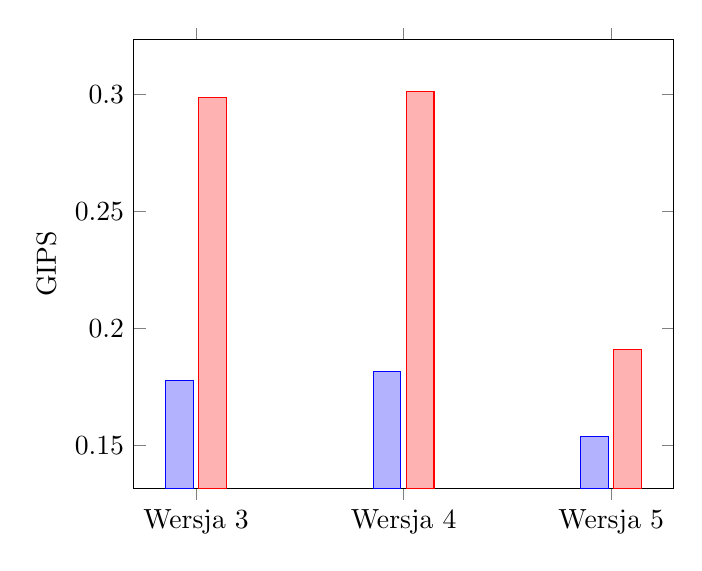
\begin{tikzpicture}
\begin{axis}[
  ybar,%=5pt,
  ylabel=GIPS,
  %ymode=log,
  log origin=infty,
  enlargelimits=0.15,
  xtick=data,
  symbolic x coords={Wersja 3, Wersja 4, Wersja 5}
]
\addplot 
  coordinates {%
    (Wersja 3, 0.1775)
    (Wersja 4, 0.1815)
    (Wersja 5, 0.1538)
  };

\addplot 
  coordinates {%
    (Wersja 3, 0.2989)
    (Wersja 4, 0.3013) 
    (Wersja 5, 0.1909)
  };

\end{axis}
\end{tikzpicture}
}
\end{minipage}
\qquad
\begin{minipage}[c]{0.46\textwidth}
\centering

\resizebox{\textwidth}{!}{%
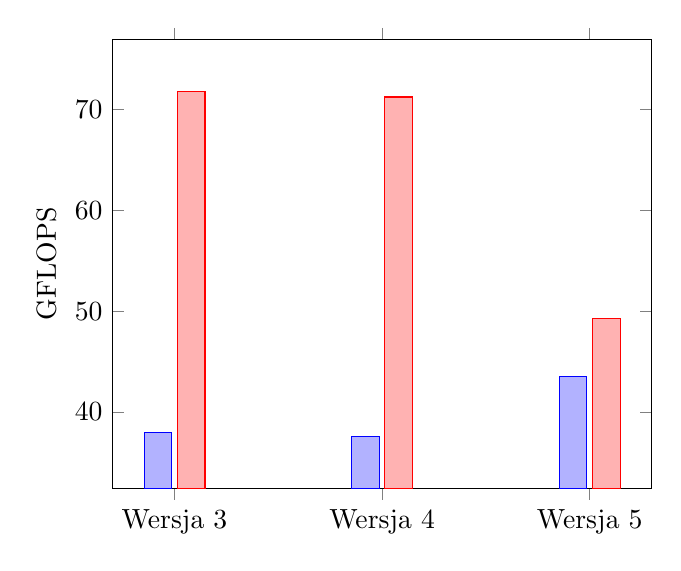
\begin{tikzpicture}
\begin{axis}[
  ybar,%=5pt,
  ylabel=GFLOPS,
  %ymode=log,
  log origin=infty,
  enlargelimits=0.15,
  xtick=data,
  symbolic x coords={Wersja 3, Wersja 4, Wersja 5}
]
\addplot 
  coordinates {%
    (Wersja 3, 37.938)
    (Wersja 4, 37.583)
    (Wersja 5, 43.520)
  };

\addplot 
  coordinates {%
    (Wersja 3, 71.812)
    (Wersja 4, 71.269) 
    (Wersja 5, 49.314)
  };

\end{axis}
\end{tikzpicture}
}

\vspace{18pt}

\resizebox{\textwidth}{!}{%
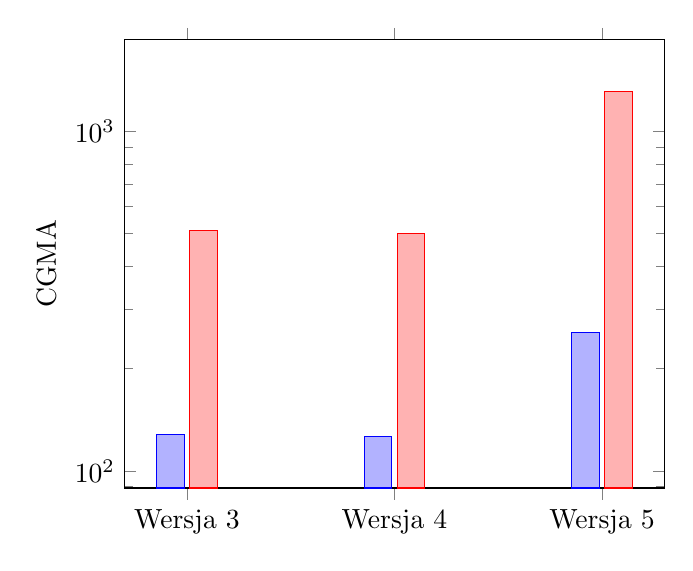
\begin{tikzpicture}
\begin{axis}[
  ybar,%=5pt,
  ylabel=CGMA,
  ymode=log,
  log origin=infty,
  enlargelimits=0.15,
  xtick=data,
  symbolic x coords={Wersja 3, Wersja 4, Wersja 5}
]
\addplot 
  coordinates {%
    (Wersja 3, 127.760)
    (Wersja 4, 126.499)
    (Wersja 5, 255.393)
  };

\addplot 
  coordinates {%
    (Wersja 3, 510.723)
    (Wersja 4, 500.764) 
    (Wersja 5, 1310.720)
  };

\end{axis}
\end{tikzpicture}
}
\end{minipage}

\caption{Porównanie drugiej grupy rozwiązań -- macierz 640x640.}

\end{figure}
